%% -*- mode: latex; mode: flyspell -*-
\documentclass[12pt, letter]{article}

%% Class name and Assignment number
%%
\newcommand{\courseName}{ECE 435 Medical~Image~Processing}
\newcommand{\assignName}{Assignment~4}

%% Packages
\usepackage{amsmath,amsfonts,amssymb,amsthm,dsfont}
\usepackage{graphicx}
\usepackage[bookmarks=false]{hyperref}
\usepackage{color}
\usepackage{lipsum}
\usepackage{amsmath}
\usepackage{booktabs}

%% Paper format
\usepackage{geometry}
\geometry{
    letterpaper,
    %% total={216mm,279mm}, %< NSERC size
    margin=2.00cm,     %< default
    %% margin=1.87cm,       %< NSERC tightest
}

%% Headers and footers
\usepackage[explicit]{titlesec}
\newpagestyle{titlesec_assignment}{
  \sethead{\courseName}{}{\assignName}\setfoot{}{\thepage}{}
  \headrule
  %% \footrule
}

\begin{document}

%% Set header and footer
\pagestyle{titlesec_assignment}

%% Title
\title{\courseName\\\assignName}
\author{Yiping Wang V00894385}
\maketitle

\paragraph{Question 2:} Test the algorithm on the image ``angiogram.tif''. You will provide the following results:
\begin{enumerate}
    \item The binarized image with the value of the threshold at convergence
    \item The histogram of ‘angiogram.tif’ image with the value of the threshold specified on it.
    \item A table containing the value of the threshold at every iteration before reaching convergence.
\end{enumerate}

\paragraph{Answer:}
The following results are obtained when tolerance is set to $\mathbf{10^{-8}}$. The initial estimate of the threshold is randomly selected from the element of the image.  

The binarized image with threshold at convergence of $\mathbf{103.9122}$ and the histogram of ``angiogram.tif'' image with the threshold at convergence of $\mathbf{103.9122}$ shows in Figure~\ref{fig:q2-1}. Table~1 shows the value of the threshold at every iteration before reaching convergence.

\begin{figure}
    \centering
    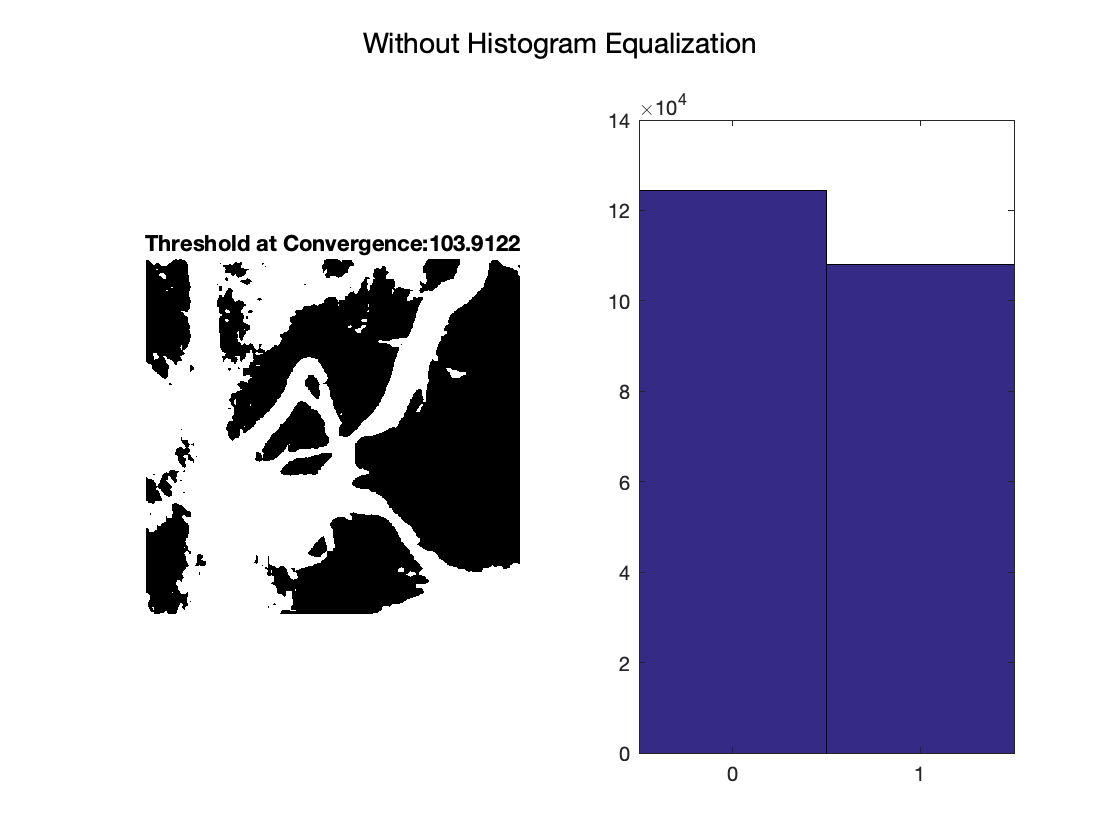
\includegraphics[width=14cm]{q2-1.png}
    \caption{Binarized Image and Its Histogram when Threshold at Convergence of 103.9122}
    \label{fig:q2-1}
\end{figure}

\begin{center}
\begin{tabular}{llr}  
\toprule
\multicolumn{2}{c}{Table 1} \\
\cmidrule(r){1-2}
Iteration   & Threshold Value \\
\midrule
1      & 43 \\
2 & 71.4590 \\
3  & 82.2945 \\
4     & 88.1546 \\
5 & 92.6288 \\
6 & 95.8906 \\
7 & 97.8611 \\
8 & 97.8611 \\
9 & 99.3100 \\
10 & 100.7898 \\
11 & 101.6115 \\
12 & 102.3741 \\
13 & 103.1515 \\
14 & 103.9122 \\
\bottomrule
\label{table:q2-1}
\end{tabular}    
\end{center}

Moreover, after invoking the function a few times, we obtain a different segmentation result since the initial estimate of the thresholds are different. 

The binarized image with threshold at convergence of $\mathbf{137.5802}$ and the histogram of ``angiogram.tif'' image with the threshold at convergence of $\mathbf{137.5802}$ shows in Figure~\ref{fig:q2-2}. Table~2 shows the value of the threshold at every iteration before reaching convergence.

\begin{figure}
    \centering
    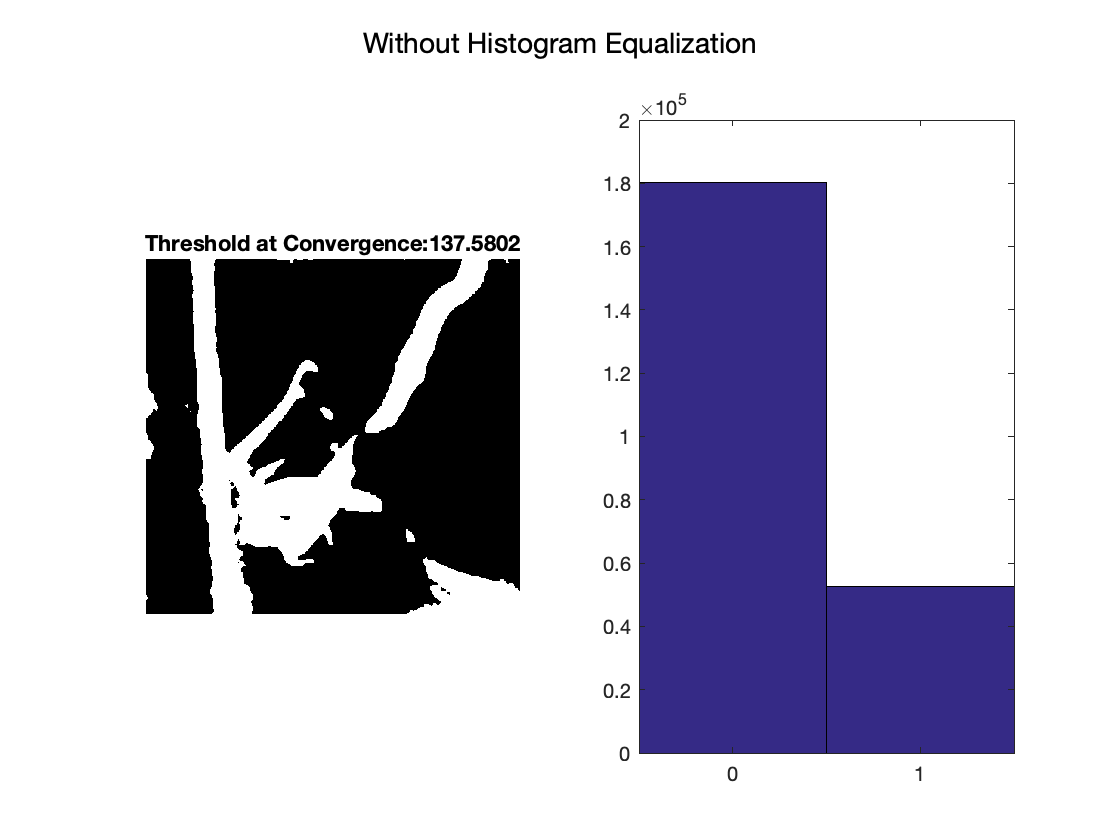
\includegraphics[width=14cm]{q2-2.png}
    \caption{Binarized Image and Its Histogram when Threshold at Convergence of 137.5802}
    \label{fig:q2-2}
\end{figure}

\begin{center}
\begin{tabular}{llr}  
\toprule
\multicolumn{2}{c}{Table 2} \\
\cmidrule(r){1-2}
Iteration   & Threshold Value \\
\midrule
1      & 168 \\
2 & 137.5802 \\

\bottomrule
\label{table:q2-2}
\end{tabular}    
\end{center}

\paragraph{Question 3:} Apply histogram equalization to ‘angiogram.tif’. You may choose to work with the Matlab \textbf{histeq} function. Next, apply the same thresholding algorithm to the equalized image. Compute the new threshold, and the new binarized images

The binarized image with threshold at convergence of $\mathbf{105.6698}$ and the histogram of ``angiogram.tif'' image with the threshold at convergence of $\mathbf{105.6698}$ shows in Figure~\ref{fig:q3-1}. Table~3 shows the value of the threshold at every iteration before reaching convergence.

\begin{figure}
    \centering
    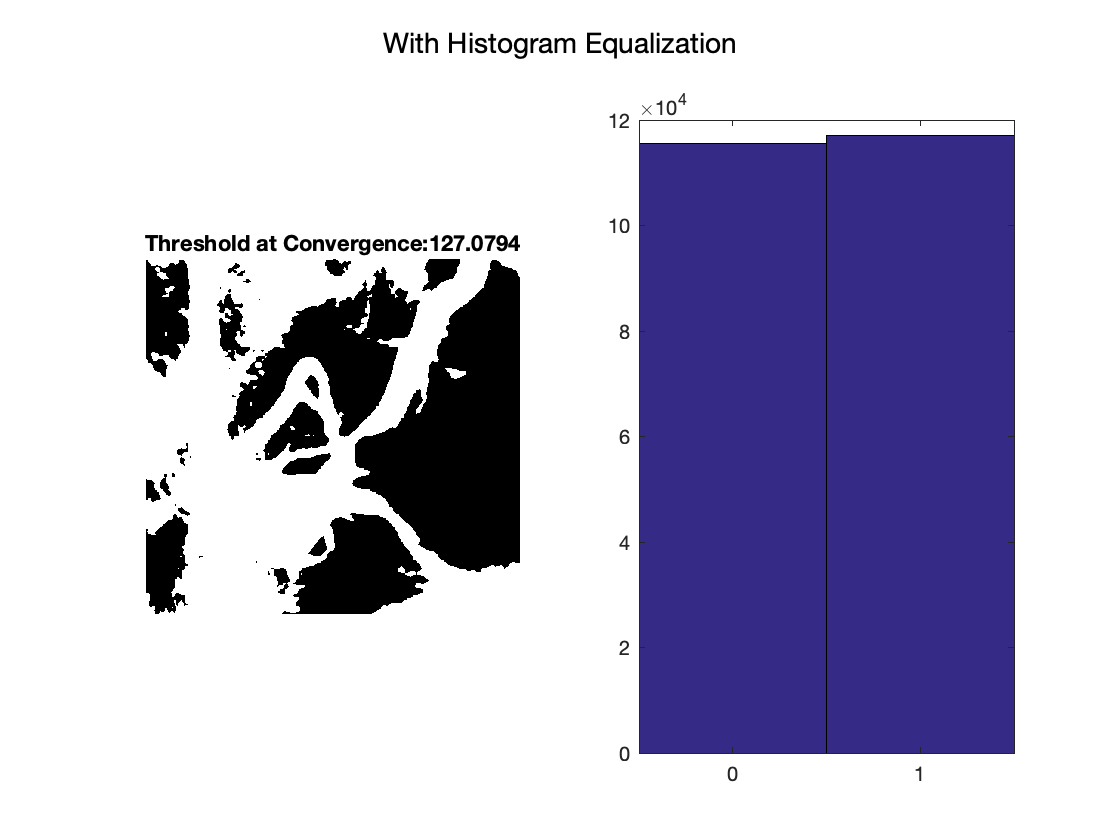
\includegraphics[width=14cm]{q3-1.png}
    \caption{Binarized Image and Its Histogram when Threshold at Convergence of 105.6698}
    \label{fig:q3-1}
\end{figure}

\begin{center}
\begin{tabular}{llr}  
\toprule
\multicolumn{2}{c}{Table 3} \\
\cmidrule(r){1-2}
Iteration   & Threshold Value \\
\midrule
1 & 28 \\
2 & 78.6122 \\
3 & 102.8717 \\
4 & 115.3512 \\
5 & 121.2035 \\
6 & 125.9473 \\
7 & 127.0794 \\

\bottomrule
\label{table:q2-2}
\end{tabular}    
\end{center}

Moreover, after invoking the function a few times, we obtain a different segmentation result since the initial estimate of the thresholds are different. 

The binarized image with threshold at convergence of $\mathbf{172.2672}$ and the histogram of ``angiogram.tif'' image with the threshold at convergence of $\mathbf{172.2672}$ shows in Figure~\ref{fig:q3-2}. Table~4 shows the value of the threshold at every iteration before reaching convergence.

\begin{figure}
    \centering
    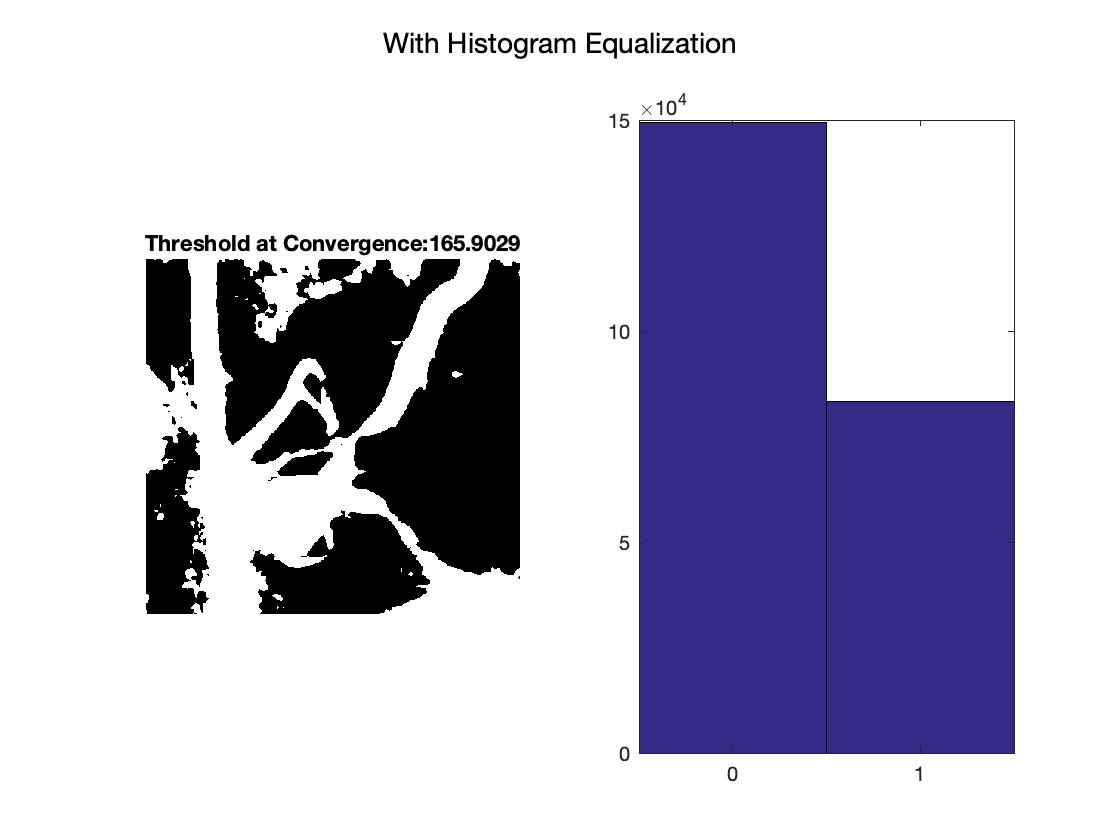
\includegraphics[width=14cm]{q3-2.png}
    \caption{Binarized Image and Its Histogram when Threshold at Convergence of 172.2672}
    \label{fig:q3-2}
\end{figure}

\begin{center}
\begin{tabular}{llr}  
\toprule
\multicolumn{2}{c}{Table 4} \\
\cmidrule(r){1-2}
Iteration   & Threshold Value \\
\midrule
1 & 202 \\
2 & 172.2672 \\

\bottomrule
\label{table:q2-2}
\end{tabular}    
\end{center}

\paragraph{Question 4: } Compare and discuss the results obtained by optimal thresholding on the original image, and on the image pre-processed with histogram equalization.
\end{document}


%%% Local Variables:
%%% mode: latex
%%% TeX-master: t
%%% End:
